\chapter{Coherent Current Oscillations}
\label{chap:cco}



Before analyzing the oscillatory dynamics observed in the simulations, it is useful to clarify the terminology used in this chapter. In the present work we refer to the field-free oscillatory response of the electronic current as coherent current oscillations (CCO). Closely related behavior is widely known in spectroscopy under the term free induction decay (FID).

The concept of free induction decay was originally introduced in nuclear magnetic resonance (NMR), where a short excitation pulse creates a coherent macroscopic magnetization. After the driving field is removed, the magnetization continues to evolve freely and produces an oscillatory signal whose amplitude gradually decreases due to dephasing of the underlying microscopic degrees of freedom. An analogous phenomenon occurs in optical spectroscopy: an ultrashort laser pulse can create a coherent superposition of quantum states, giving rise to a macroscopic polarization that subsequently evolves in the absence of the external field and decays as phase coherence is lost.

In semiconductors excited by few-femtosecond optical pulses, the pump field generates interband coherence between valence- and conduction-band states. This coherence corresponds to a macroscopic polarization and is accompanied by an electronic current. After the excitation pulse has vanished, the coherent superposition continues to evolve freely with frequencies determined by the interband transition energies. As a result, the macroscopic current exhibits oscillations in the field-free regime. Their decay reflects the gradual loss of phase coherence due to two distinct mechanisms: homogeneous dephasing caused by scattering processes and inhomogeneous dephasing originating from the dispersion of transition energies across the Brillouin zone.

Although this behavior is formally analogous to optical free induction decay, the observable analyzed in this work is the electric current rather than the polarization. For this reason we introduce the term coherent current oscillations (CCO). The terminology emphasizes that the measured quantity in the simulations is the current response and that the oscillations arise from coherent evolving of electronic states. In this sense, CCO can be regarded as the current analogue of free induction decay: both phenomena originate from the free evolution of a coherently prepared electronic state, but CCO specifically refers to the oscillatory current signal generated by interband coherence in solids.

Adopting this terminology is particularly convenient in the present context. The pump–probe configuration used in the simulations naturally yields the time-dependent current as the primary observable, and its oscillatory component provides direct access to the coherence properties of the electronic system. As will be shown below, analyzing the CCO signal allows a quantitative separation of homogeneous and inhomogeneous dephasing mechanisms and establishes a direct connection between coherence decay and transport relaxation in disordered media.


\section{Minimal Bloch-Basis Description: Semiconductor Bloch Equations}

To connect the RT-TDDFT observables to a compact analytical picture, we employ the standard Bloch-basis density-matrix formulation of the semiconductor Bloch equations (SBE) \cite{HaugKoch2009,RossiKuhn2002}. In a minimal two-band model (valence $v$, conduction $c$), for each crystal momentum $\mathbf{k}$ we introduce

\begin{equation}
f_c(\mathbf{k},t)=\rho_{cc}(\mathbf{k},t), \qquad
f_v(\mathbf{k},t)=\rho_{vv}(\mathbf{k},t), \qquad
p_{\mathbf{k}}(t)=\rho_{cv}(\mathbf{k},t),
\end{equation}

where $\rho_{nm}(\mathbf k,t)$ is the density matrix in the Bloch basis.
The diagonal elements $\rho_{cc}$ and $\rho_{vv}$ correspond to the electron
and hole populations, while the off-diagonal element $\rho_{cv}$ describes
the microscopic interband polarization.


The transition frequency is

\begin{equation}
\omega_{cv}(\mathbf{k})=\frac{E_c(\mathbf{k})-E_v(\mathbf{k})}{\hbar},
\end{equation}

where $E_{c(v)}(\mathbf{k})$ is the energy dispersion. The light–matter coupling can be written through the Rabi frequency

\begin{equation}
\Omega_{\mathbf{k}}(t)=\frac{1}{\hbar}\,\mathbf{E}(t)\cdot \mathbf{d}_{cv}(\mathbf{k}),
\end{equation}

where the interband dipole matrix element is defined as
\begin{equation}
\mathbf d_{cv}(\mathbf k)
=
\langle u_{c\mathbf k} | e \cdot \mathbf r | u_{v\mathbf k} \rangle,
\end{equation}

where $u_{c\mathbf k}$ and $u_{v\mathbf k}$ are the periodic parts of the Bloch
functions corresponding to the conduction and valence bands, respectively.

In the absence of scattering, the SBE read \cite{HaugKoch2009,RossiKuhn2002}

\begin{align}
\dot p_{\mathbf{k}}(t)
&=
-i\omega_{cv}(\mathbf{k})\,p_{\mathbf{k}}(t)
-i\Omega_{\mathbf{k}}(t)\,\big[f_c(\mathbf{k},t)-f_v(\mathbf{k},t)\big],
\\
\dot f_c(\mathbf{k},t)
&=
2\,\mathrm{Im}\!\left[\Omega_{\mathbf{k}}^*(t)\,p_{\mathbf{k}}(t)\right],
\qquad
\dot f_v(\mathbf{k},t)=-\dot f_c(\mathbf{k},t).
\end{align}

After the pump pulse, $\Omega_{\mathbf{k}}(t)=0$, and

\begin{equation}
\dot f_c(\mathbf{k})=0, \qquad \dot p_{\mathbf{k}}=-i\omega_{cv}(\mathbf{k})p_{\mathbf{k}}
\end{equation}

which gives 

\begin{equation}
p_{\mathbf{k}}(t)=p_{\mathbf{k}}(0)\,e^{-i\omega_{cv}(\mathbf{k})t}.
\end{equation}
% Thus, within a RT-TDDFT simulation without disorder, one has formally infinite lifetimes


The parameters $T_1$ and $T_2^*$ characterize two distinct relaxation processes of an excited electronic system. The time $T_1$ (population relaxation time) describes the decay of carrier populations toward equilibrium through processes such as recombination or energy relaxation. In contrast, total effective dephasing time $T_2^*$ characterizes the decay of phase coherence between quantum states, i.e., the loss of the off-diagonal elements of the density matrix that determine the interband polarization.

Within the RT-TDDFT framework used in this work, no explicit dissipative channels such as carrier recombination, electron–phonon scattering, or other irreversible relaxation mechanisms are included. As a result, population relaxation is absent and one formally has $T_1=\infty$. The dephasing time $T_2^*$, however, remains finite due to dephasing mechanisms. In a perfectly periodic system, the decay of the macroscopic polarization arises from inhomogeneous dephasing caused by the dispersion of interband transition frequencies $\omega_{cv}(\mathbf{k})$ across the Brillouin zone. In the presence of structural disorder, an additional mechanism contributes: elastic scattering of electronic states in both the valence and conduction bands, which leads to homogeneous dephasing and further accelerates the decay of coherence.


% Since no irreversible channel is present, 

% \begin{equation}
% T_2=\infty,\qquad T_1=\infty,
% \end{equation}


\section{Interband Coherence and Inhomogeneous Dephasing}


The macroscopic interband polarization is

\begin{equation}
P(t)=\sum_{\mathbf{k}} d_{cv}(\mathbf{k})\,p_{\mathbf{k}}(t),
\end{equation}

and the interband current is $J_{\mathrm{inter}}(t)=dP/dt$.
After the pump pulse,

\begin{equation}
p_{\mathbf{k}}(t)=p_{\mathbf{k}}(0)\,e^{-i\omega_{cv}(\mathbf{k})t}.
\end{equation}

Although each microscopic coherence is perfectly phase coherent, the macroscopic polarization

\begin{equation}
P(t)=\sum_{\mathbf{k}} A(\mathbf{k})\,e^{-i\omega_{cv}(\mathbf{k})t}
\end{equation}

decays due to phase dispersion of $\omega_{cv}(\mathbf{k})$. For a Gaussian wave packet centered at $\mathbf{k}_0$ with width $\Delta k$,

\begin{equation}
P(t)\propto e^{-i\omega_0 t}\exp\!\left[-\frac{(\Delta\omega\,t)^2}{2}\right],
\qquad
\Delta\omega\simeq |\nabla_{\mathbf{k}}\omega_{cv}|\,\Delta k.
\end{equation}

This defines the inhomogeneous dephasing time

\begin{equation}
T_{\mathrm{inh}}=\frac{1}{\Delta\omega}.
\end{equation}

In silicon, such dispersion-driven decay on the few-femtosecond scale is consistent with attosecond measurements of interband polarization dynamics \cite{Schultze2014Si,Lucchini2016Science}. 

% Importantly, this decay is not a finite microscopic $T_2$, but rather phase mixing across the excited $\mathbf{k}$ region.

\section{Static Disorder: Homogeneous Dephasing}

When static disorder is introduced, elastic scattering modifies the SBE via collision integrals \cite{HaugKoch2009,Mahan2000}. In Born \cite{AshcroftMermin,Mahan2000} and effective-mass approximation  \cite{PhysRev.97.869},

\begin{equation}
W_{\mathbf{k}\to\mathbf{k}'}^{c(v)}
=
\frac{2\pi}{\hbar} n_i |\delta V_{\mathbf{k}\mathbf{k}'}^{c(v)}|^2
\delta(E_{c(v)}(\mathbf{k})-E_{c(v)}(\mathbf{k}')),
\end{equation}

where $n_i$ is the concentration of the scattering centers, $|\delta V_{\mathbf{k}\mathbf{k}'}|^2$ is defined by \ref{eq:delta_V}, the indices $c$ and $v$ refer to the conduction and valence bands, respectively and $E_{c(v)}(\mathbf{k})$ is the energy dispersion. The single-particle scattering rate is

\begin{equation}
\Gamma_{c(v)}(\mathbf{k})=\sum_{\mathbf{k}'} W_{\mathbf{k}\to\mathbf{k}'}^{c(v)}.
\label{eq:gamma_def}
\end{equation}

The interband dephasing time satisfies \cite{Peropadre_2013}

\begin{equation}
\frac{1}{T_2(\mathbf{k})}
=
\frac{1}{2}\big[\Gamma_c(\mathbf{k})+\Gamma_v(\mathbf{k})\big].
\label{eq:t2_gamma}
\end{equation}

Thus, each microscopic coherence decays exponentially,

\begin{equation}
p_{\mathbf{k}}(t)=p_{\mathbf{k}}(0)\,e^{-i\omega_{cv}(\mathbf{k})t}\,e^{-t/T_2(\mathbf{k})}.
\end{equation}

The macroscopic polarization envelope becomes approximately

\begin{equation}
P(t)\sim e^{-t/T_2}\exp\!\left[-\frac{t^2}{2T_{\mathrm{inh}}^2}\right].
\end{equation}




\section{Angular Factor and the Relation between $T_2$ and $\tau_m$}

Static disorder also relaxes intraband currents by randomizing momentum. However, the time scale governing current decay is not the same as the single-particle lifetime. The transport (momentum) relaxation time is defined by inserting an angular weight:
\begin{equation}
\frac{1}{\tau_{m}^{c(v)}(\mathbf{k})}
=
\sum_{\mathbf{k}'}
W_{\mathbf{k}\to\mathbf{k}'}^{c(v)}\left(1-\cos\theta_{\mathbf{k}\mathbf{k}'}\right),
\label{eq:tau_m}
\end{equation}
where $\theta_{\mathbf{k}\mathbf{k}'}$ is the scattering angle. The factor $(1-\cos\theta)$ encodes the fact that small-angle (forward) scattering barely changes the velocity direction.

It is useful to define the \emph{angular factor}
\begin{equation}
\alpha_{c(v)}(\mathbf{k})\equiv
\frac{\sum_{\mathbf{k}'} W_{\mathbf{k}\to\mathbf{k}'}^{c(v)}\left(1-\cos\theta_{\mathbf{k}\mathbf{k}'}\right)}
{\sum_{\mathbf{k}'} W_{\mathbf{k}\to\mathbf{k}'}^{c(v)}},
\label{eq:alpha_def}
\end{equation}
which satisfies $0<\alpha_{c(v)}(\mathbf{k})< 2$ and is typically $\alpha\sim 1$ for isotropic short-range disorder, while $\alpha\ll 1$ for forward-peaked scattering (e.g.\ screened Coulomb potentials). Combining Eqs.~\eqref{eq:gamma_def}, \eqref{eq:tau_m}, and \eqref{eq:alpha_def} yields a direct relation between the single-particle rate and the transport time,
\begin{equation}
\Gamma_{c(v)}(\mathbf{k})=\frac{1}{\alpha_{c(v)}(\mathbf{k})\,\tau_{m}^{c(v)}(\mathbf{k})}.
\end{equation}
Substituting into Eq.~\eqref{eq:t2_gamma} gives the connection we discussed:
\begin{equation}
\frac{1}{T_2(\mathbf{k})}
=
\frac{1}{2}\left[
\frac{1}{\alpha_c(\mathbf{k})\,\tau_{m,c}(\mathbf{k})}
+
\frac{1}{\alpha_v(\mathbf{k})\,\tau_{m,v}(\mathbf{k})}
\right].
\label{eq:t2_tau_m}
\end{equation}
Two limits summarize the physics. If scattering is isotropic so that $\alpha\approx 1$ and if $\tau_{m,c}\approx \tau_{m,v}$ (which is true for the Born approximation and plane waves in the formula \ref{eq:delta_V}), then $T_2$ and $\tau_m$ are comparable. If scattering is strongly forward-peaked ($\alpha\ll 1$), then $T_2$ can be much shorter than $\tau_m$: coherence decays rapidly even though the current persists relatively longer.

For a finite $\mathbf{k}$-distribution, the intraband current generally becomes a superposition of exponentials,
\begin{equation}
J_{\mathrm{intra}}(t)=e\sum_{\mathbf{k}} v_c(\mathbf{k})\,\delta f_c(\mathbf{k},0)\,e^{-t/\tau_m(\mathbf{k})}+\cdots,
\end{equation}
so a single $\tau_m$ may not describe the entire waveform. Nevertheless, Eq.~\eqref{eq:tau_m} identifies which microscopic part of the impurity scattering controls the decay of the pump-induced drift/anisotropy.




\section{Observed Coherent Current Oscillations Dynamics}

\begin{figure}[h!]
    \centering
    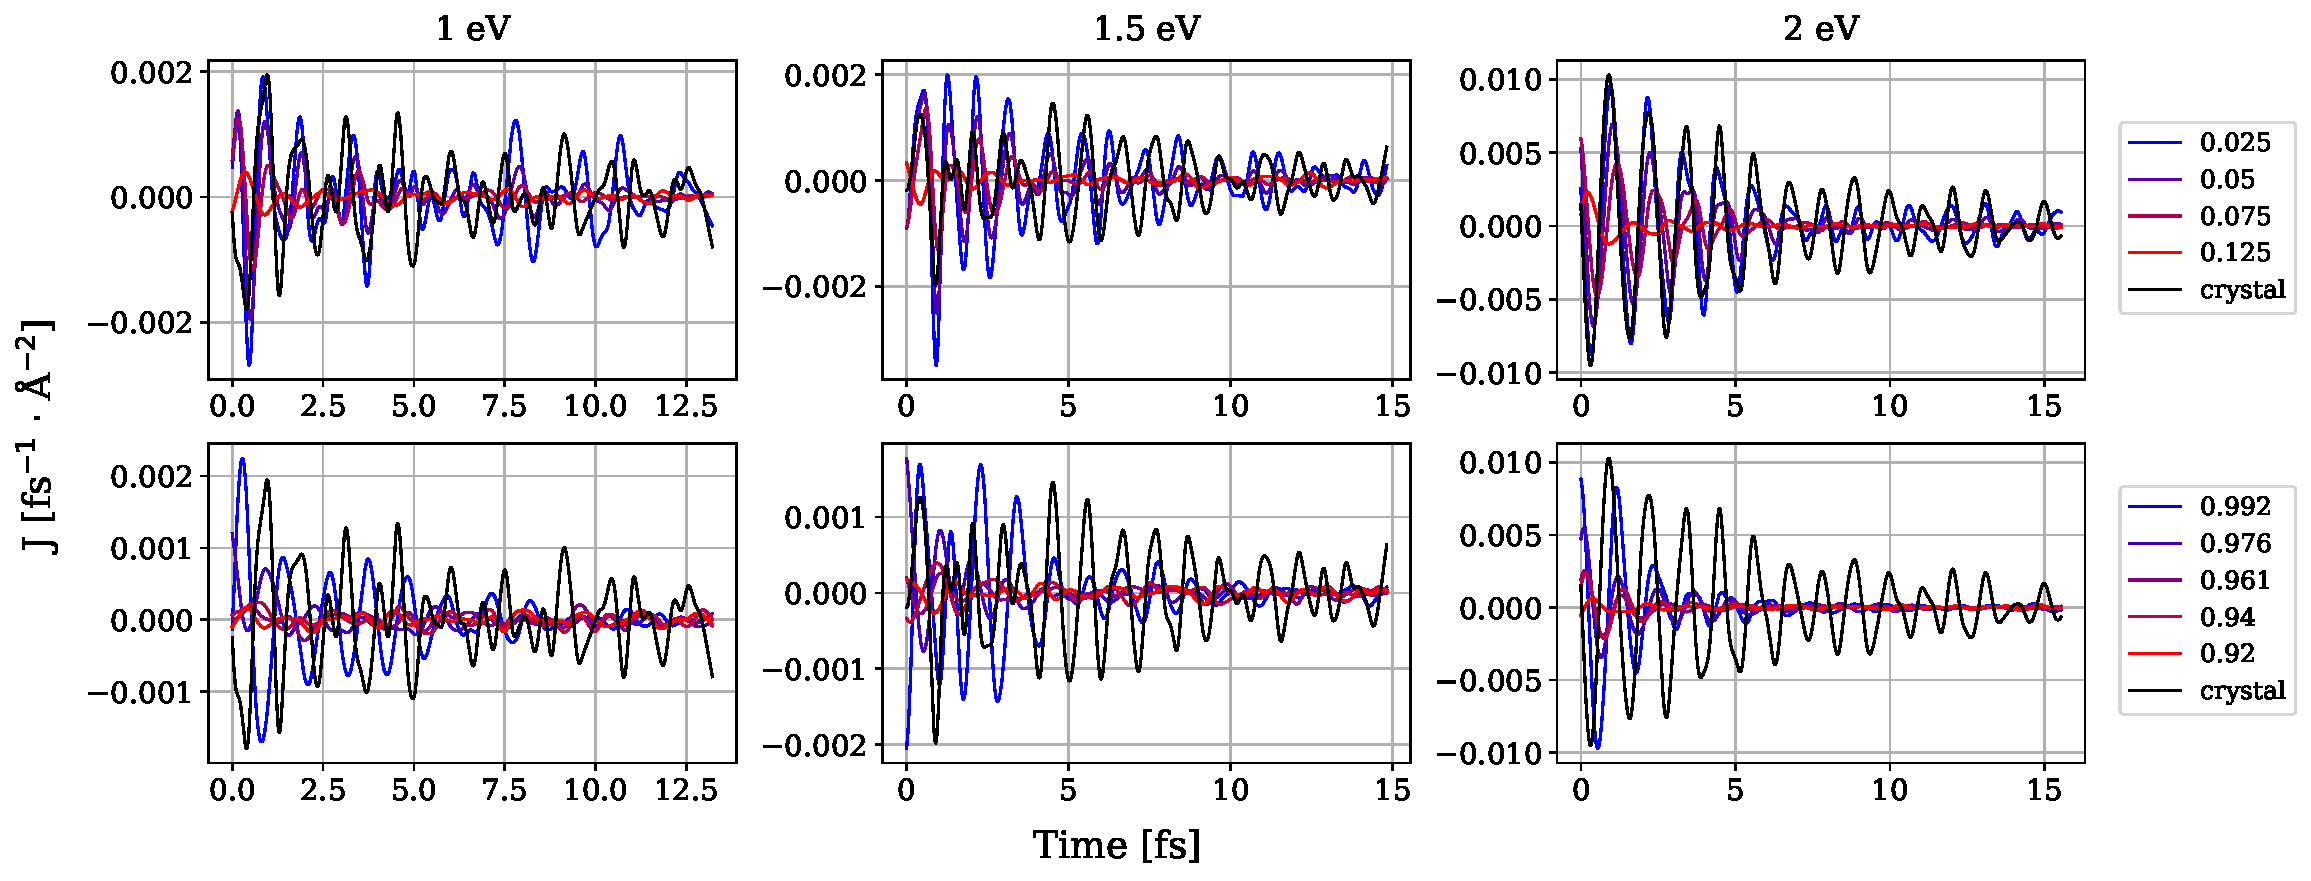
\includegraphics[width=1\linewidth]{all_pdf/cco/pdf/coherent_current_oscillations.pdf}
    \caption{Field-free coherent current oscillations $J_z(t)$ after the pump pulse for different disorder strengths and pump photon energies. The column caption in eV indicates the carrier frequency of the pump pulse. The top row represents displacement disorder, whereas the bottom row represents amorphous disorder.}
    \label{fig:cco_time}
\end{figure}

Figure~\ref{fig:cco_time} shows the CCO along the $z$-axis after the pump pulse, i.e., in the absence of an external field. In a perfect crystal, the decay of the macroscopic signal is governed solely by inhomogeneous dephasing caused by dispersion of the transition frequency $\omega_{cv}(\mathbf{k})$ over the excited region of reciprocal space. As discussed above, this mechanism leads to an approximately Gaussian envelope characterized by the inhomogeneous time $T_{\mathrm{inh}}$.

When static disorder is introduced, an additional homogeneous exponential decay channel appears due to elastic scattering. In that case, the macroscopic polarization and the corresponding interband current envelope can be written schematically as

\begin{equation}
J_z(t) \sim 
\exp\!\left(-\frac{t}{T_2}\right)
\exp\!\left(-\frac{t^2}{2T_{\mathrm{inh}}^2}\right),
\end{equation}

where $T_2$ is the homogeneous dephasing time associated with impurity scattering, while $T_{\mathrm{inh}}$ describes dispersion-driven phase mixing. The total effective dephasing time $T_2^*$ is therefore determined by both mechanisms, and in the regime where the exponential decay dominates one may approximate

\begin{equation}
\frac{1}{T_2^*} \equiv \frac{1}{\tau_{\mathrm{coh}}^z}
\approx
\frac{1}{T_2}
+
\frac{1}{T_{\mathrm{inh}}^{\mathrm{eff}}}.
\end{equation}

Although in the case where we have several spectral peaks, the attenuation shape is not Gaussian, such a division into different dephasing channels will still be justified, since exponential attenuation is uniform.

It is clearly seen in Fig.~\ref{fig:cco_time} that the oscillations decay more rapidly as disorder increases, indicating a progressive reduction of $T_2$. Moreover, in the pumping regime closest to linear absorption (carrier frequency 2 eV), the oscillations are spectrally cleaner and exhibit a more regular phase evolution. In contrast, strongly nonlinear pumping (1 eV and 1.5 eV) generates a broader and more complex distribution of microscopic phases, which enhances inhomogeneous contributions and leads to a more irregular macroscopic waveform.

\begin{figure}[h!]
    \centering
    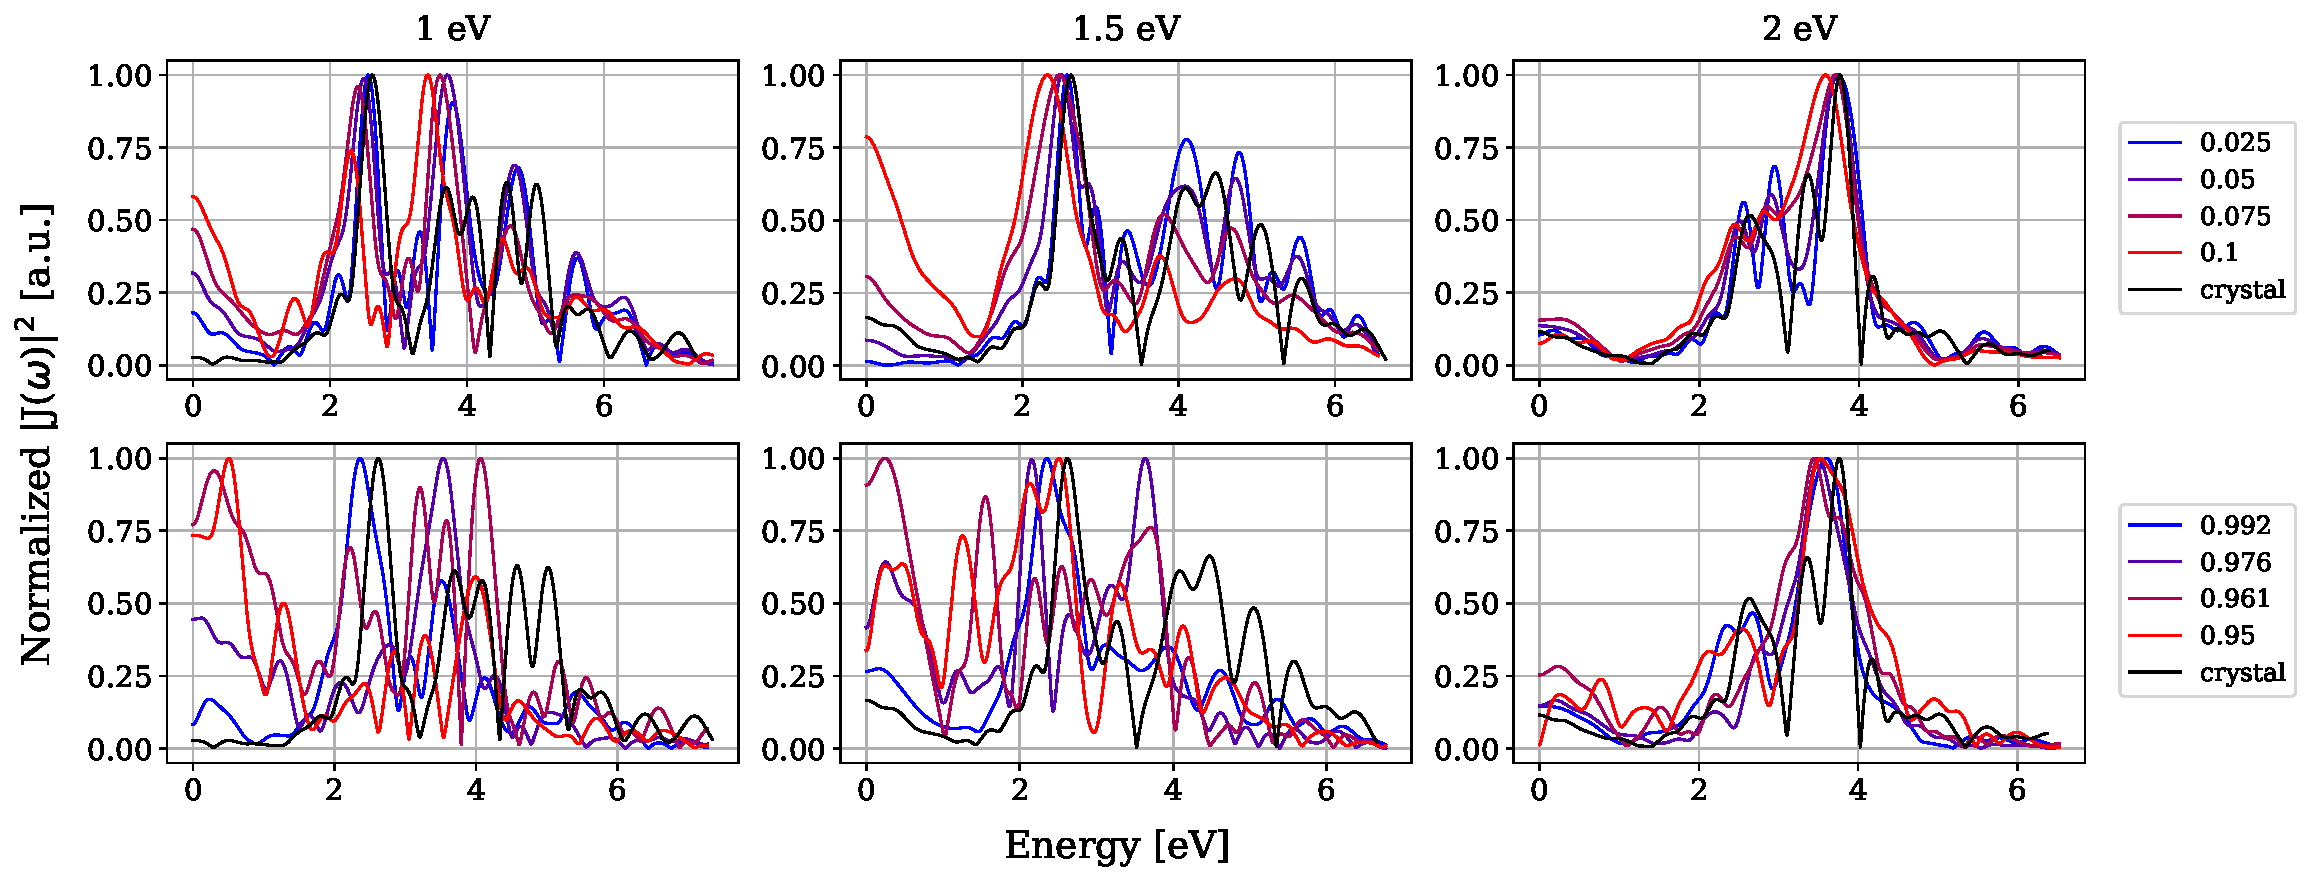
\includegraphics[width=1\linewidth]{all_pdf/cco/pdf/coherent_current_oscillations_spectrum.pdf}
    \caption{Power spectrum of coherent current oscillations $|J_z(\omega)|^2$ for increasing disorder. The column caption in eV indicates the carrier frequency of the pump pulse. The top row represents displacement disorder, whereas the bottom row represents amorphous disorder.}
    \label{fig:cco_spectrum}
\end{figure}

The corresponding spectra in Fig.~\ref{fig:cco_spectrum} show a systematic red shift with increasing disorder, consistent with band-gap reduction. Spectral broadening is also evident. For amorphous disorder under nonlinear pumping, the spectrum becomes significantly more irregular compared to displacement disorder, indicating abrupt activation of transitions that are symmetry-forbidden in the crystalline limit. For nearly linear pumping at 2 eV, the spectral modifications are much weaker, reflecting the more selective excitation of states near the band edge.

\section{Dephasing Times Decomposition}

\begin{figure}[h!]
    \centering
    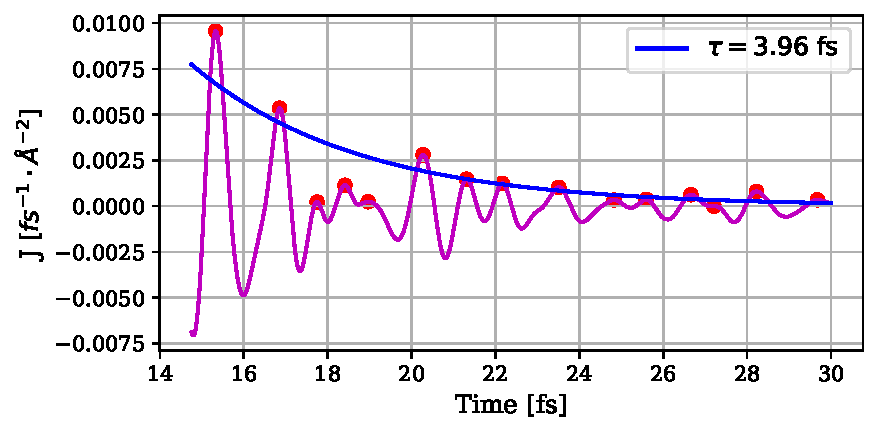
\includegraphics[width=0.7\linewidth]{all_pdf/additional/fid/3_fid_z_c333_amorphous_0.95_s0.050_r18_k16_a1_i804_t9_p1.5d11_1d12.pdf}
    \caption{Example of a coherent current oscillation signal used for coherence-time analysis.}
    \label{fig:cco_signal}
\end{figure}

Figure~\ref{fig:cco_signal} shows a representative CCO waveform for a displacement disorder of 0.05 Å. Our goal is to separate the homogeneous exponential decay from the residual inhomogeneous contribution and to test whether the two mechanisms can be decomposed additively at the level of decay rates.

\begin{figure}[h!]
    \centering
    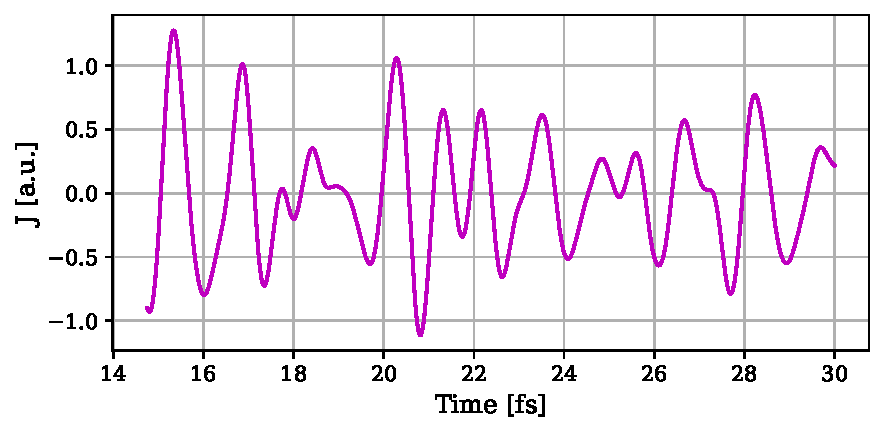
\includegraphics[width=0.67\linewidth]{all_pdf/additional/fid/3_normalized_fid_z_c333_amorphous_0.95_s0.050_r18_k16_a1_i804_t9_p1.5d11_1d12.pdf}
    \caption{Exponentially normalized coherent current oscillation signal.}
    \label{fig:cco_norm}
\end{figure}

To isolate the non-exponential component, we normalize the signal by the homogeneous decay factor associated with the transport time $\tau_m$ obtained from the probe-direction Drude analysis:

\begin{equation}
\tilde{J}_z(t)
=
J_z(t)\,e^{(t-t^*)/\tau_m}.
\end{equation}

The normalized signal $\tilde{J}_z(t)$, shown in Fig.~\ref{fig:cco_norm}, should primarily contain inhomogeneous phase mixing if the homogeneous part is indeed governed by the same scattering time $\tau_m$.

\begin{figure}[h!]
    \centering
    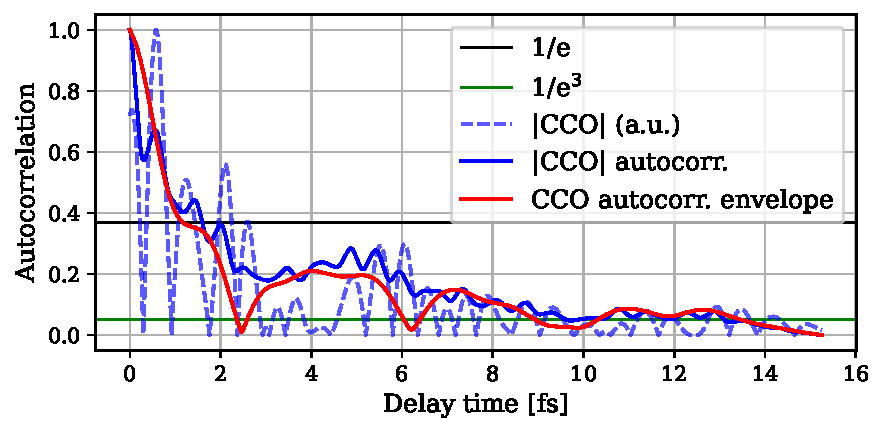
\includegraphics[width=0.8\linewidth]{all_pdf/additional/fid/3_autocorrelation_of_abs_fid_z_c333_amorphous_0.95_s0.050_r18_k16_a1_i804_t9_p1.5d11_1d12.pdf}
    \caption{Autocorrelation of the CCO signal and its Hilbert-envelope used for coherence-time extraction.}
    \label{fig:cco_autocorr}
\end{figure}

To quantify coherence, we compute the autocorrelation of the absolute signal,

\begin{equation}
C(\tau)=\int_{t_0}^{\infty} |J_z(t)|\,|J_z(t+\tau)|\,dt,
\qquad \tau\ge 0.
\end{equation}

We then construct the analytic signal via the Hilbert transform $\mathcal{H}$:

\begin{equation}
\mathcal{C}(\tau)=C(\tau)+i\,\mathcal{H}[C](\tau),
\end{equation}

and define the envelope

\begin{equation}
A(\tau)=|\mathcal{C}(\tau)|.
\end{equation}

Following coherence theory concepts \cite{MandelWolf1995}, we define the coherence decay time as

% \begin{equation}
% \tau_{\mathrm{coh}}^z
% =
% \frac{2\left(\int_{0}^{\infty} A(\tau)\,d\tau\right)^2}
% {\int_{0}^{\infty} A^2(\tau)\,d\tau}.
% \end{equation}

\begin{equation}
\tau_{\mathrm{coh}} \equiv 2 \int_0^\infty \left| \frac{A(\tau)}{A(0)} \right|^2 \, d\tau
\end{equation}

The prefactor 2 accounts for restricting the analysis to positive delays.

\begin{figure}[h!]
    \centering
    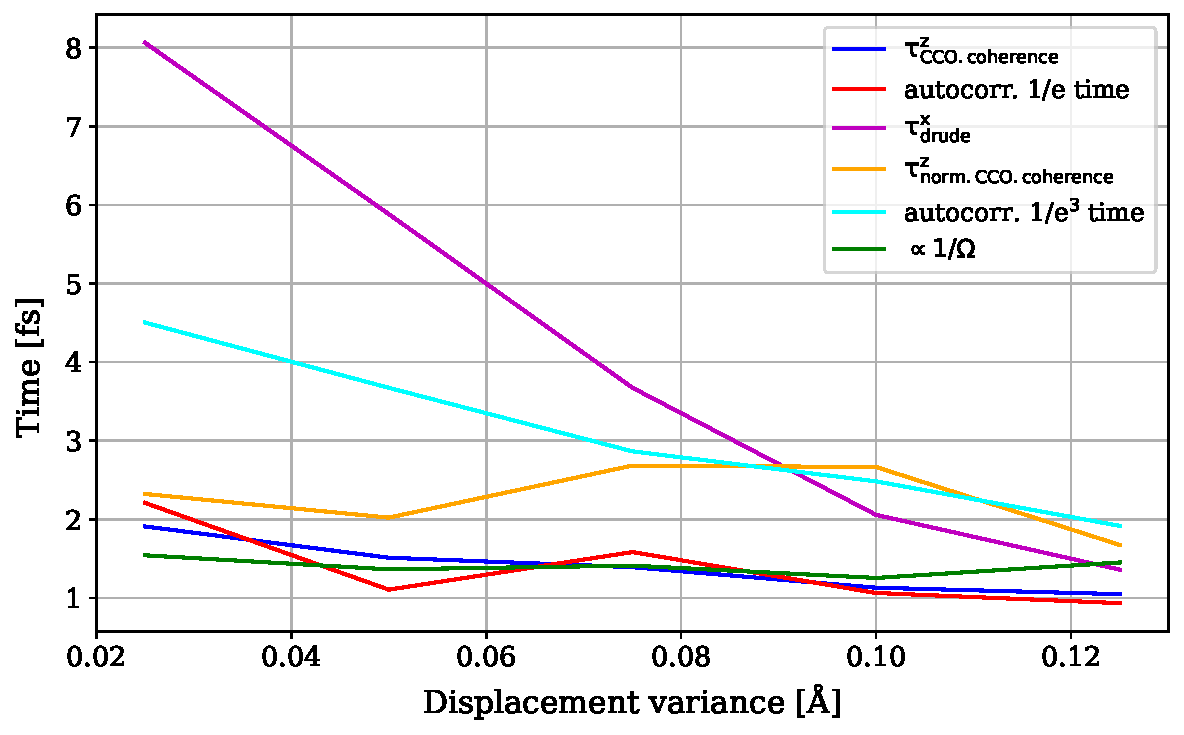
\includegraphics[width=0.7\linewidth]{all_pdf/cco/pdf/сomparison_of_coherence_times.pdf}
    \caption{Comparison of different coherence-time definitions and their relation to the transport time.}
    \label{fig:cco_compare}
\end{figure}

Figure~\ref{fig:cco_compare} compares various coherence-time definitions. The most relevant quantity is $\tau_{\mathrm{coh}}^z$, representing the total dephasing time of the field-free CCO signal. Also shown is the coherence decay time extracted from the exponentially normalized signal, isolating inhomogeneous effects. The transport time $\tau_m$ is plotted for reference. Remarkably, the inverse spectral width (obtained from the squared autocorrelation integral) correlates strongly with $\tau_{\mathrm{coh}}^z$, indicating that spectral broadening and temporal dephasing are directly linked. The coherence decay time determined at the $1/e$ level for the autocorrelation of the signal module gives a good similarity to $\tau_{\mathrm{coh}}^z$. What is also evident is that the definition at the $1/e^3$ level allows us to approximately extract a longer-range correlation due to exponential decay for displacement variances below 0.08 (while exponential decay takes longer than inhomogeneous decay). The comparison suggests the presence of two characteristic time scales: a shorter time arising from inhomogeneous broadening and a longer
time reflecting homogeneous scattering.

\begin{figure}[h!]
    \centering
    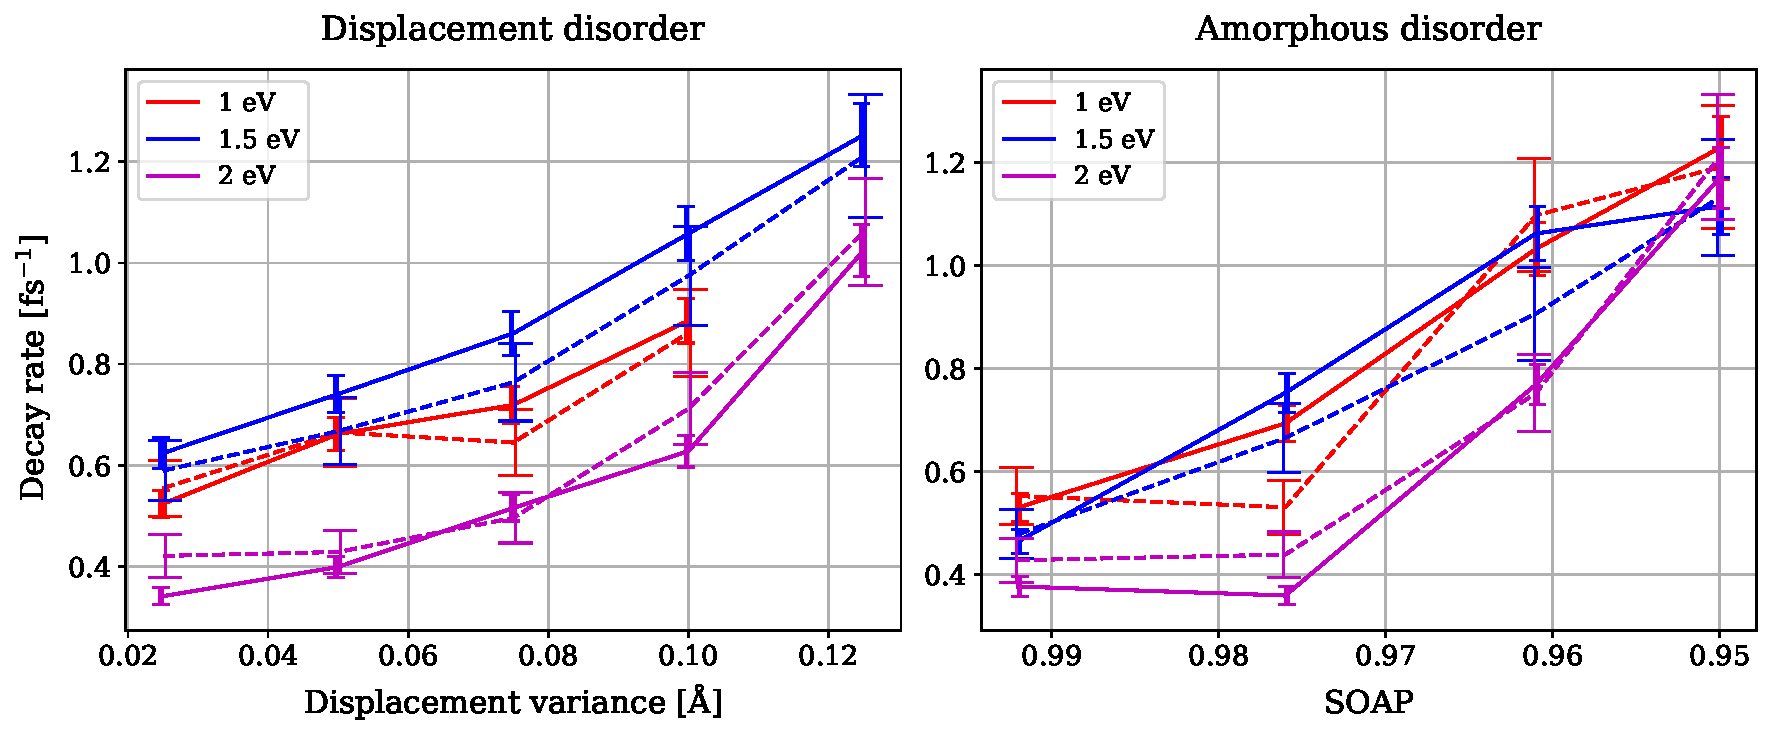
\includegraphics[width=1\linewidth]{all_pdf/cco/pdf/cco_decay_rate_decomposition.pdf}
    \caption{Test of additivity of decay rates: comparison of $1/\tau_{\mathrm{coh}}^z$ with $1/\tau_m + 1/\tau_{\mathrm{coh}}^{z,\mathrm{norm}}$.}
    \label{fig:cco_decomposition}
\end{figure}

Finally, Fig.~\ref{fig:cco_decomposition} tests the relation

\begin{equation}
\frac{1}{\tau_{\mathrm{coh}}^z}
=
\frac{1}{\tau_m}
+
\frac{1}{\tau_{\mathrm{coh}}^{z,\mathrm{norm}}}.
\end{equation}

Here $\tau_{\mathrm{coh}}^{z,\mathrm{norm}}$ is the coherence decay time for the normalized CCO signal. For nearly all points, the error bars overlap. This shows that the homogeneous part of \, CCO decay is governed by the same elastic scattering time that controls intraband transport. Consequently, the effective angular factor in the transport time definition is close to unity, indicating nearly isotropic impurity scattering in the bias-disorder model considered here.